\subsection{Разработка схемы алгоритма работы с программным средством}
\label{sec:design:app}

Алгоритм работы программного средства представлен на рисунке~\ref{fig:design:app:diagram}.
На данной схеме виден алгоритм работы приложением.
При входе в приложение открывается пользователю должен предоставляться выбор списка сущностей, с которыми он может работать (также возможно отображение одно из списков по умолчанию с возможностью перехода к остальным).
Как видно из рисунка~\ref{fig:design:app:diagram} за взаимодействием с пользователем отвечают три модуля: модуль работы с транзакциями, модуль работы со счетами и модуль работы с категориями.

\begin{sidewaysfigure}
    \centering
    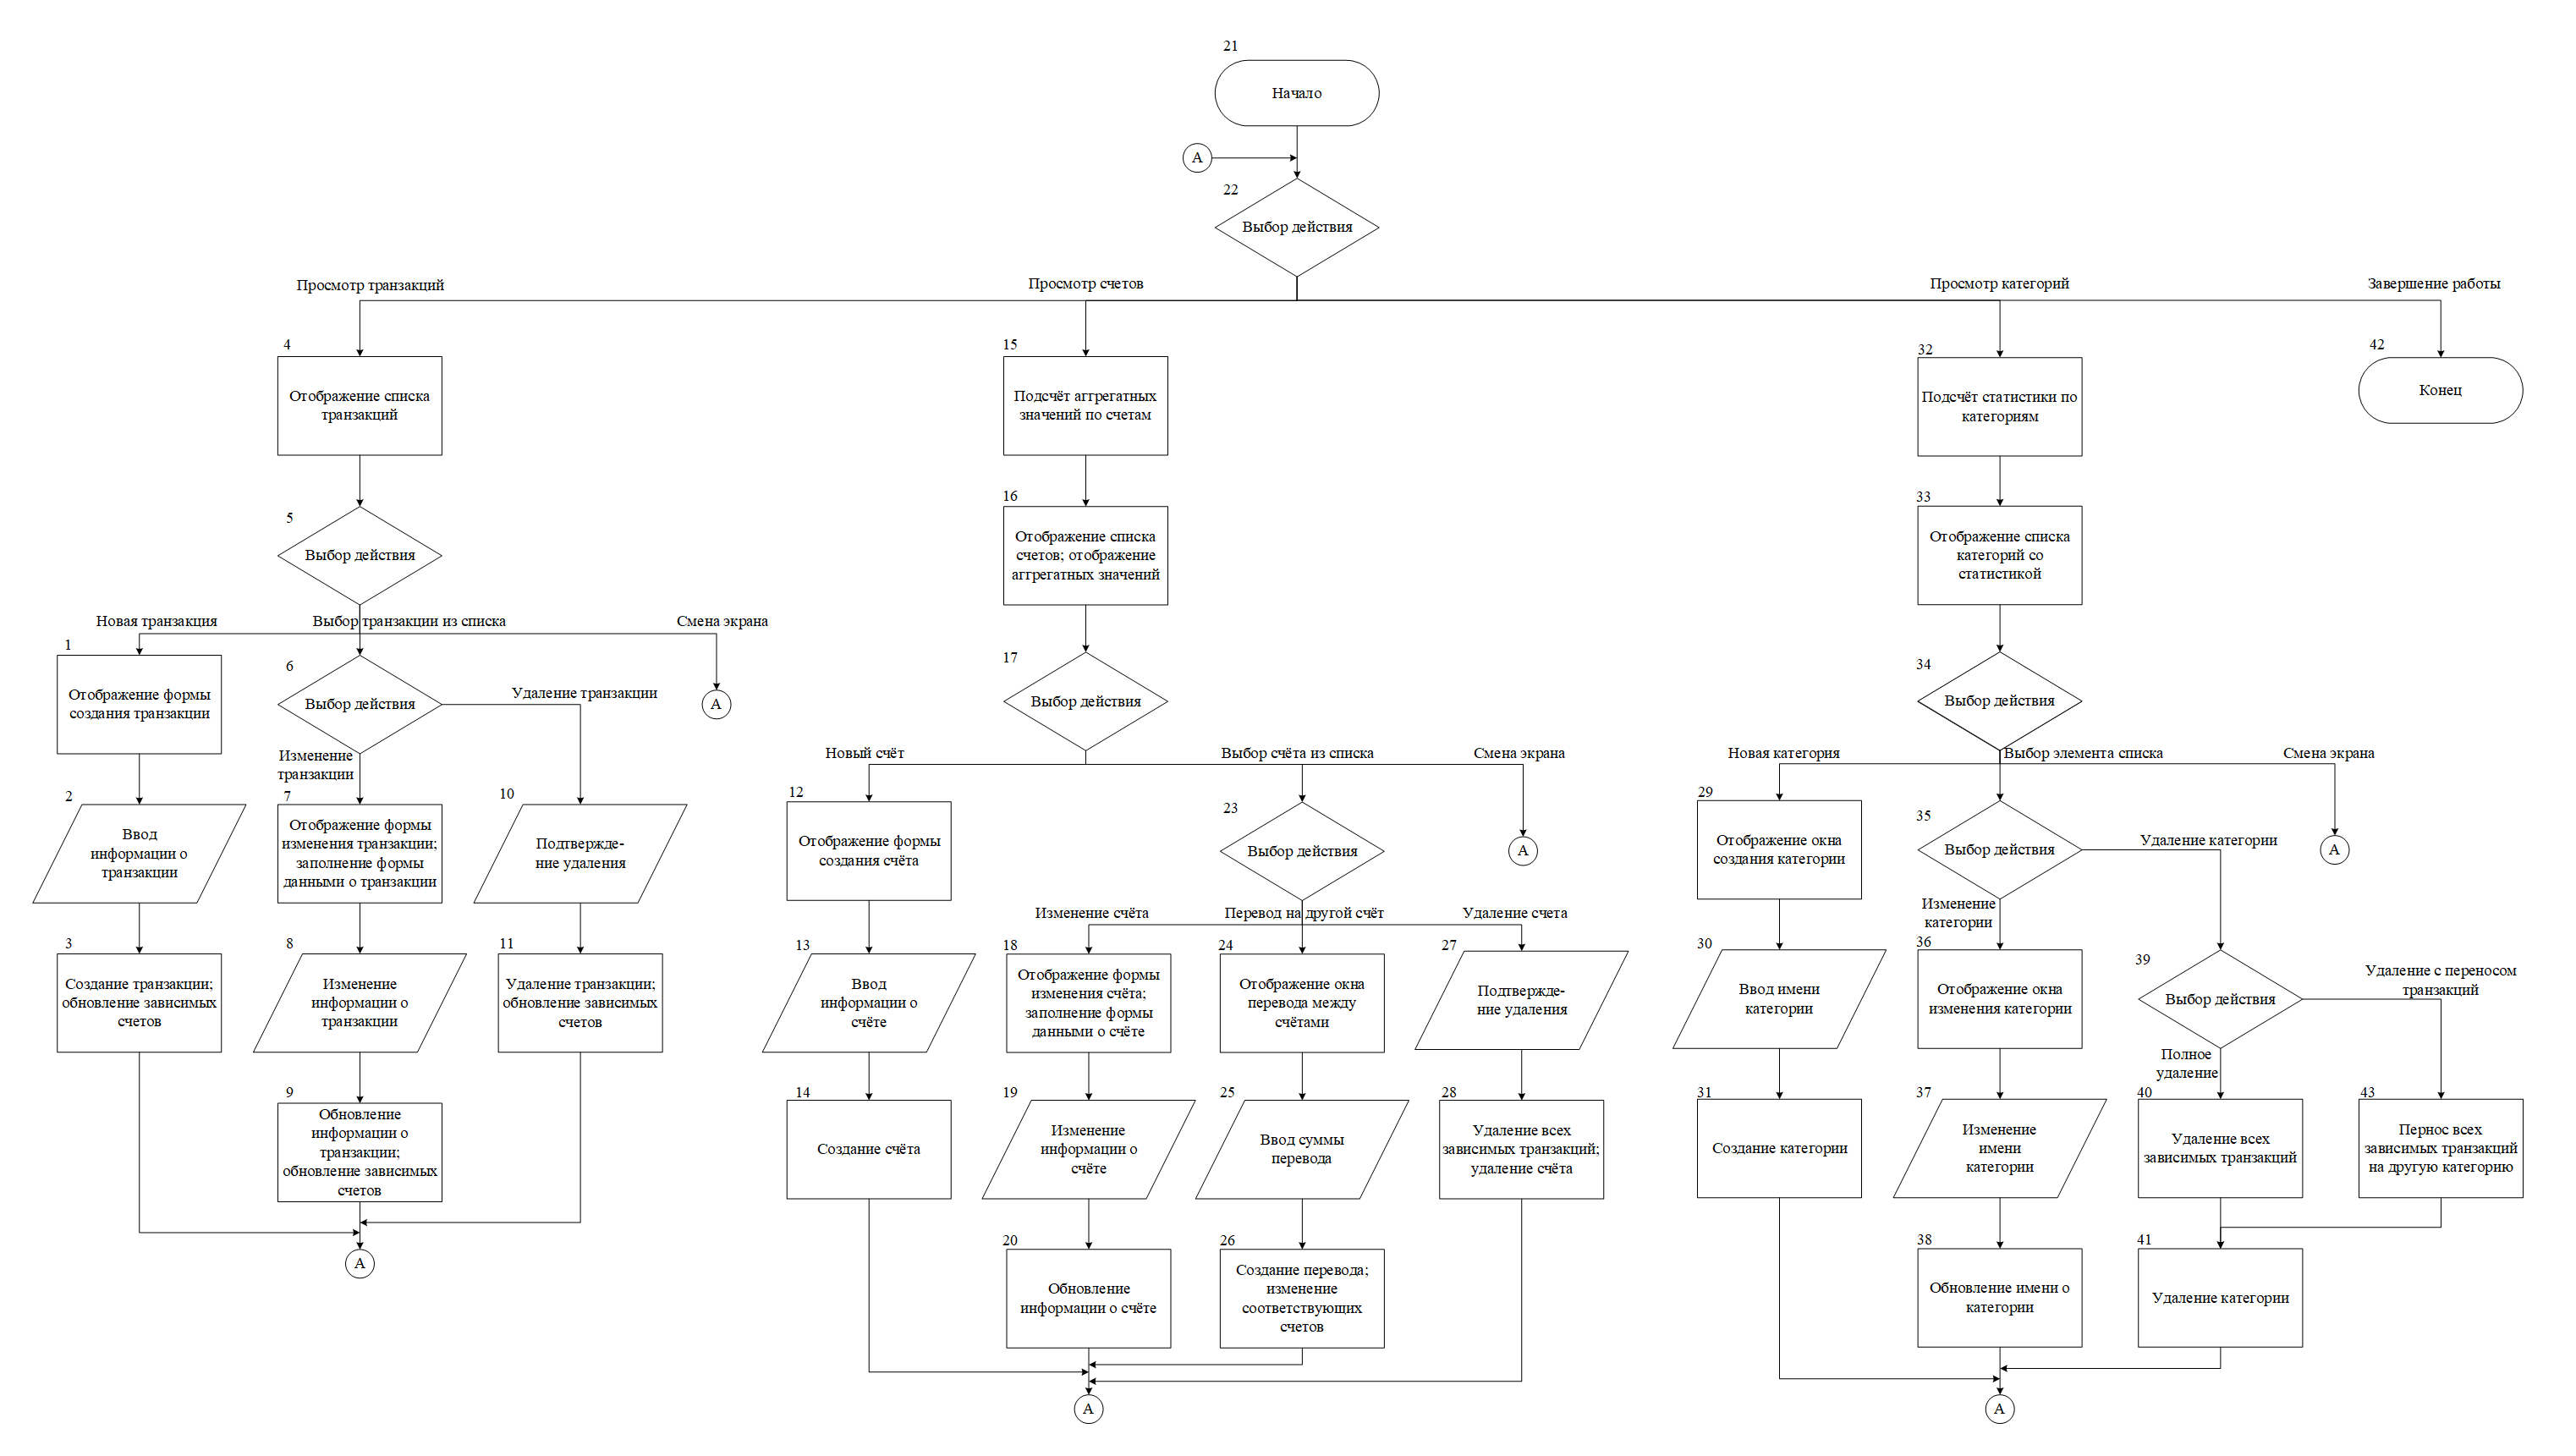
\includegraphics[scale=0.275]{3_4_app_diagram.png}
    \caption{Схема программного средства}
    \label{fig:design:app:diagram}
\end{sidewaysfigure}

